\documentclass[utf8, 11pt]{beamer}
\usepackage{verbatim}
\usepackage{color}
\usepackage{graphicx}
\usepackage{alltt}
%\usepackage{hyperref}
%\hypersetup{colorlinks=true, urlcolor=cyan}
\hypersetup{urlcolor=cyan}

\mode<presentation>
{
  \usetheme{default}
}

\usepackage[english, russian]{babel}
\usepackage{graphicx}
\usepackage{colortbl}
\usepackage{listings}

\newcommand{\rsb}{\cellcolor[gray]{0.85}}
\newcommand{\nam}[1]{\texttt{#1}}

\setbeamertemplate{navigation symbols}{} 

\author[ ]{Карташов Д. А., Савенко С. А.}

\title[Virtual HSM]{Разработка виртуального HSM для платформы Linux}


\institute[ ]
{
  Parallels Lab SPbAU
}

\date{ }

\subject{Talks}

\useoutertheme{infolines}
\setbeamertemplate{headline}{}

\begin{document}

\begin{frame}
  \titlepage
\end{frame}

\begin{frame}{Введение}

Криптография в приложениях:
\begin{itemize}
\item хранение секретных данных
\item вычисления с их использованием
\end{itemize}

\vspace*{\fill}

Проблемы безопасности:
\begin{itemize}
\item компрометация секретных данных
\end{itemize}

\vspace*{\fill}

Решение:
\begin{itemize}
\item исключить попадание секретных данных на диск и/или в память компьютера
\end{itemize}

\vspace*{\fill}

\end{frame}

\begin{frame}{Цели и задачи проекта}

\begin{block}{Цель}
Разработать решение, предоставляющее функциональность HSM в виртуальном окружении
\end{block}

\vspace*{\fill}

\begin{block}{Задачи}
\begin{itemize}
\item поиск и анализ существующих решений;
\item изучение стандартов HSM;
\item изучение приложений, поддерживающих HSM;
\item разработка прототипа VHSM.
\end{itemize}
\end{block}

\end{frame}

\begin{frame}{Существующие решения}

Существующие решения:
\begin{itemize}
\item Amazon CloudHSM:

\url{http://aws.amazon.com/cloudhsm/}
\end{itemize}

\vspace*{\fill}

Стандарты HSM:
\begin{itemize}
\item pkcs\#11:

\url{http://www.rsa.com/rsalabs/node.asp?id=2133}
\end{itemize}

\vspace*{\fill}

%\includegraphics[width=0.32\textwidth]{img1}
Использование HSM в приложениях:
\begin{center}
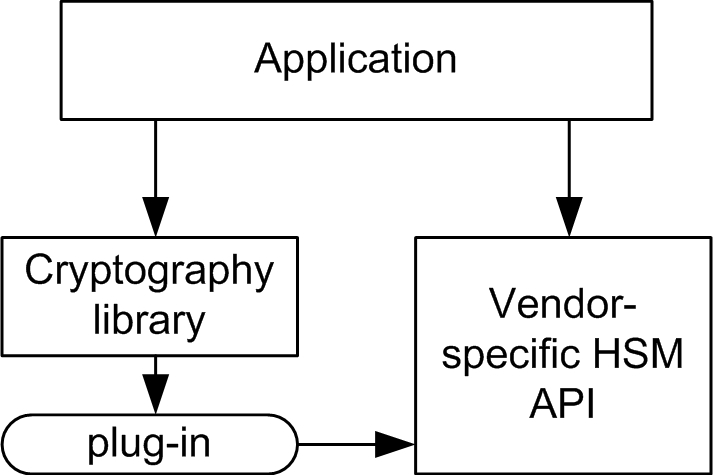
\includegraphics[scale=0.75]{img1-2}
\end{center}

\end{frame}

\begin{frame}{Общая архитектура решения}
\begin{center}
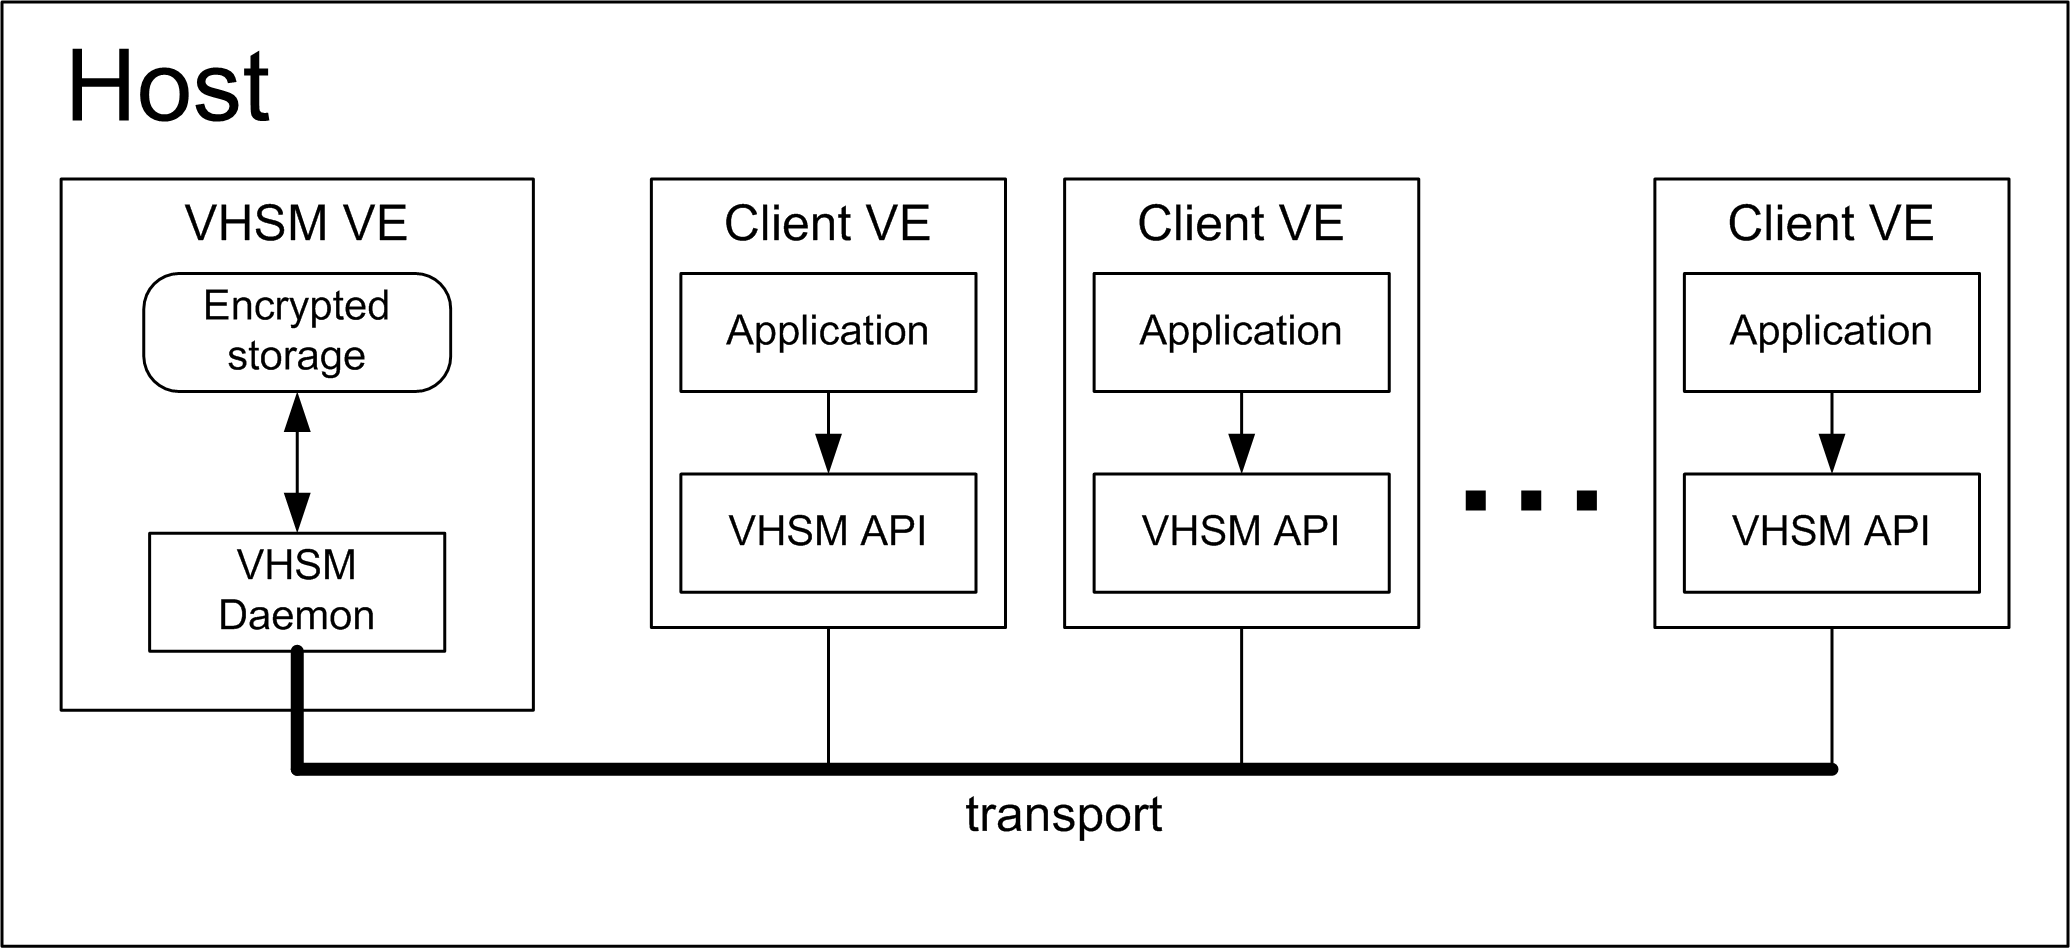
\includegraphics[width=0.95\paperwidth]{img2}
\end{center}
\end{frame}

\begin{frame}{Основные компоненты}
\begin{itemize}
\item {\bf Transport}
	\begin{itemize}
		\item пересылка сообщений
		\item идентификация контейнеров
	\end{itemize}
\item {\bf VHSM API}
	\begin{itemize}
		\item передача запросов на выполнение криптографических операций через транспорт
		\item получение результатов операций
	\end{itemize}
\item {\bf VHSM daemon}
	\begin{itemize}
		\item аутентификация
		\item выполнение криптографических операций с использованием секретных данных
	\end{itemize}
\item {\bf Encrypted storage}
	\begin{itemize}
		\item хранение секретных данных пользователя
	\end{itemize}
\end{itemize}

\end{frame}

\begin{frame}[fragile]
\frametitle{Transport}
\begin{itemize}
\item протокол --- \texttt{Google Protobuf}
\item реализован на файловой системе
	\begin{itemize}
	\item структура каталогов:
\begin{lstlisting}
transport
|__ containers
|   |__ CNT1
|   |   |__ in
|   |   |__ out
|   |__ CNT2
|       |__ in
|       |__ out
|__ vhsm
    |__ in
    |__ out
\end{lstlisting}
	\end{itemize}
\end{itemize}
\end{frame}

\begin{frame}[fragile]
\frametitle{VHSM API}

\lstset{language=C++, basicstyle=\ttfamily\scriptsize}
\begin{itemize}
\item управление сессиями
\begin{lstlisting}
vhsm_rv vhsm_login(vhsm_session session,
                   vhsm_credentials credentials);
vhsm_rv vhsm_logout(vhsm_session session);
\end{lstlisting}

\item управление ключами
\begin{lstlisting}
vhsm_rv vhsm_key_mgmt_delete_key(vhsm_session session,
                                 vhsm_key_id key_id);
vhsm_rv vhsm_key_mgmt_create_key(vhsm_session session,
                                 vhsm_key key);
\end{lstlisting}

\item хэширование и МАС
\begin{lstlisting}
vhsm_rv vhsm_mac_init(vhsm_session session,
                      vhsm_mac_method method);
vhsm_rv vhsm_mac_update(vhsm_session session,
                        unsigned char const * data_chunk,
                        unsigned int chunk_size);
vhsm_rv vhsm_mac_end(vhsm_session session,
                     unsigned char * mac_ptr,
                     unsigned int * mac_size_ptr);
\end{lstlisting}
\end{itemize}
\end{frame}

\begin{frame}[fragile]{VHSM daemon и encrypted storage}

\begin{itemize}
\item вычисление криптографических функций
\item хранение пользовательских данных
	\begin{itemize}
	\item генерация ключа для шифрования с использованием секрета пользователя
	\item шифрование AES в режиме GCM
	\item реализовано на файловой системе
\begin{lstlisting}
encrypted_storage
|__ .fses_root
|__ user1
|   |__ .fses_ns
|   |   |__ .fses_ns_cf
|   |__ key1
|__ user2
    |__ .fses_ns
    |   |__ .fses_ns_cf
    |__ key1
\end{lstlisting}
	\end{itemize}
\end{itemize}
\end{frame}

\begin{frame}{OpenSSL engine}

{\bf OpenSSL engine} --- модуль расширения для OpenSSL, используемый для делегирования криптографических функций VHSM.
\begin{itemize}
\item динамический;
\item статический (встроен в \texttt{libcrypto}).
\end{itemize}

\vspace*{\fill}

Различия при использовании стандартных и нестандартных алгоритмов хэширования и шифрования:
\begin{itemize}
\item нестандартные алгоритмы могут использоваться только через унифицированные интерфейсы;
\item функциональность стандартных алгоритмов может быть перегружена по запросу пользователя.
\end{itemize}

\end{frame}

\begin{frame}{OpenSSL engine --- детали реализации}

В текущей реализации движка изменен алгоритм SHA1 так, чтобы он смог разграничить фазы вычисления HMAC и передавать в VHSM корректные данные.

\vspace*{\fill}

Минусы:
\begin{itemize}
\item алгоритм работы движка основан на текущей реализации функции HMAC в OpenSSL, и при ее изменении он станет некорректным;
\item алгоритм SHA1 ведет себя не так, как этого может ожидать пользователь. 
\end{itemize}

Плюсы:
\begin{itemize}
\item от конечного пользователя не потребуется значительных усилий по внедрению поддержки VHSM в свое приложение.
\end{itemize}

\vspace*{\fill}

\end{frame}

\begin{frame}[fragile]{OpenSSL engine --- конфигурация}

\lstset{language=C++, basicstyle=\ttfamily\scriptsize}

В файл \texttt{/etc/ssl/openssl.cnf} необходимо добавить следующие строки:
\begin{itemize}
\item в начале файла:
\begin{lstlisting}
openssl_conf = openssl_def
\end{lstlisting}
\item в конце файла:
\begin{lstlisting}
[openssl_def]
engines = engine_section
[engine_section]
test_engine = test_engine_section

[test_engine_section]
engine_id = test_engine
dynamic_path = /path/to/test_engine.so
username = user
password = password
init = 0
\end{lstlisting}

\end{itemize}

\end{frame}

\begin{frame}{Пример использования}
\begin{center}
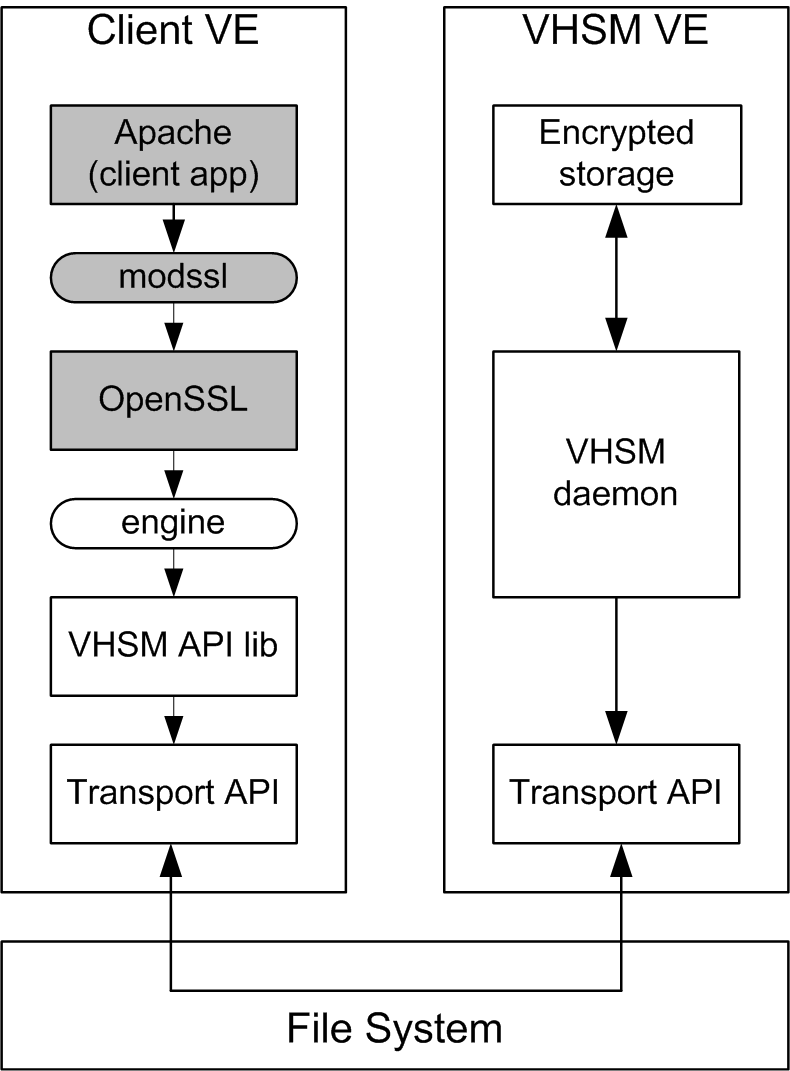
\includegraphics[scale=0.7]{img3-1}
\end{center}
\end{frame}

\begin{frame}{Итоги и планы}

Реализован прототип:
\begin{itemize}
	\item MAC
	\item хэш-функции
	\item управление ключами
	\item OpenSSL engine
\end{itemize}

\vspace*{\fill}

Планы на будущее:
\begin{itemize}
\item Повышение надёжности шифрования
\item Реализация транспорта через netlink / pipe
\item Расширение функциональности
\item Реализация системы конфигурации
\item Тестирование
\item Рефакторинг
\end{itemize}

\vspace*{\fill}

\end{frame}

\begin{frame}{Ссылки}
\begin{itemize}
\item Репозиторий проекта:

\url{https://github.com/OSLL/vhsm}

\item wiki проекта:

\url{http://osll.spb.ru/projects/vhsm/wiki}
\end{itemize}

\vspace*{\fill}

\end{frame}

\end{document}
